%%%%%%%%%%%%%%%%%%%%%%%%%%%%%%%%%%%%%%%%%%%%%%%%%%%%%%%%%%%%%%%%%%%%%%%%%%%%%%%%
%2345678901234567890123456789012345678901234567890123456789012345678901234567890
%        1         2         3         4         5         6         7         8

\documentclass[letterpaper, 10 pt, conference]{ieeeconf}  % Comment this line out if you need a4paper



%\documentclass[a4paper, 10pt, conference]{ieeeconf}      % Use this line for a4 paper

\IEEEoverridecommandlockouts                              % This command is only needed if 
                                                          % you want to use the \thanks command

\overrideIEEEmargins                                      % Needed to meet printer requirements.

%In case you encounter the following error:
%Error 1010 The PDF file may be corrupt (unable to open PDF file) OR
%Error 1000 An error occurred while parsing a contents stream. Unable to analyze the PDF file.
%This is a known problem with pdfLaTeX conversion filter. The file cannot be opened with acrobat reader
%Please use one of the alternatives below to circumvent this error by uncommenting one or the other
%\pdfobjcompresslevel=0
%\pdfminorversion=4

% See the \addtolength command later in the file to balance the column lengths
% on the last page of the document

% The following packages can be found on http:\\www.ctan.org
%\usepackage{graphics} % for pdf, bitmapped graphics files
%\usepackage{epsfig} % for postscript graphics files
%\usepackage{mathptmx} % assumes new font selection scheme installed
%\usepackage{times} % assumes new font selection scheme installed
\usepackage{amsmath} % assumes amsmath package installed
\usepackage{amssymb}  % assumes amsmath package installed
\usepackage{hyperref}


 \usepackage{easyReview}
 


\title{\LARGE \bf
Matrix Multiplication-Driven Repulsive Fields for Manipulator Kinematic Obstacle Avoidance
}


\author{
	Jakob Baumgartner$^{1}$ and Gregor Klančar$^{2}$% <-this % stops a space
%\thanks{*This work was not supported by any organization}% <-this % stops a space
%\thanks{$^{1}$Albert Author is with Faculty of Electrical Engineering, Mathematics and Computer Science,
%        University of Twente, 7500 AE Enschede, The Netherlands
%        {\tt\small albert.author@papercept.net}}%
%\thanks{$^{2}$Bernard D. Researcheris with the Department of Electrical Engineering, Wright State University,
%        Dayton, OH 45435, USA
%        {\tt\small b.d.researcher@ieee.org}}%
}


\begin{document}



\maketitle
\thispagestyle{empty}
\pagestyle{empty}


%%%%%%%%%%%%%%%%%%%%%%%%%%%%%%%%%%%%%%%%%%%%%%%%%%%%%%%%%%%%%%%%%%%%%%%%%%%%%%%%
\begin{abstract}



\end{abstract}

\add{ADD}


%%%%%%%%%%%%%%%%%%%%%%%%%%%%%%%%%%%%%%%%%%%%%%%%%%%%%%%%%%%%%%%%%%%%%%%%%%%%%%%%
\section{INTRODUCTION}

%The robots environment is modelled by discrete voxels. As the robots environment can dynamically change, we propose a method that looks at the surrounding space of the robot and calculates these direction away from all the surrounding obstacles in real time. We only look in a predefined area / perimeter arround the robot.  
%
%In 3D computer graphics, a voxel represents a value on a regular grid in three-dimensional space. Each of the voxels holds the probability value of its occupation. In case of voxel being empty it holds the value of 0, if the voxel is occupied it holds the value of non-zero, depending on our assurance of it being occupied. If it is definitly occupied it holds the value of 1. 

%Motion planning involves finding paths for manipulators through joint configurations from an initial to a goal position, respecting constraints and optimization criteria due to redundant degrees of freedom (DOF)~\cite{siciliano1990kinematic}. This redundancy allows for diverse configurations, optimizing secondary tasks like avoiding singularities and obstacles while maintaining the primary goal of reaching the End Effector (EE) target~\cite{siciliano2010robot}.
%
%Global motion planning methods search the entire configuration space for optimal paths but lack real-time applicability and smoothness~\cite{vsvestka1997motion,lavalle1998rapidly, karaman2010incremental,kuffner2000rrt,gammell2015batch}. Local methods, notably inverse kinematics and quadratic programming, offer real-time, smooth solutions but can get stuck in local minima due to their short-sighted planning approach~\cite{c29,c38,c21,c23}.
%
%The Artificial Potential Field (APF) concept by Khatib~\cite{c33}, which integrates repulsive forces for obstacle avoidance and attractive forces towards goals, has seen various improvements to mitigate issues like local minima~\cite{c40,c43,c45,c46,c47}. Recent works have adapted APF variations for manipulator motion planning, combining them with techniques like numerical Jacobians for enhanced path planning~\cite{c49,park2020trajectory}.
%
%For dynamic environments, strategies like ESDF grids, calculated directly from sensor data or occupancy grids, assist in real-time obstacle detection and avoidance~\cite{oleynikova2017voxblox,han2019fiesta,lau2010improved,rong2006jump,zhou2021egoplanner}. Our novel approach utilizes occupancy voxel grids to generate repulsive velocities, dynamically directing the robot away from obstacles based on proximity, thus enabling effective navigation in changing environments. This method ensures the robot maintains a safe distance from obstacles, with repulsive velocities adjusting in real-time to navigate the manipulator through the safest path possible.

Motion planning~\cite{c52} is a technique in robotics, that is used to calculate joint changes leading manipulators from initial to a target configuration, while addressing constraints and optimization criteria. This task is facilitated by the manipulators' redundant degrees of freedom (DOF), enabling it to undertake various configurations to not only reach their End Effector (EE) target but also optimize for secondary objectives such as obstacle avoidance and minimizing joint torques~\cite{siciliano1990kinematic}.

While global motion planning techniques provide comprehensive solutions by examining the entire configuration space, they fall short in terms of smoothness and real-time application, making them less ideal for dynamic settings~\cite{lavalle1998rapidly, gammell2015batch, karaman2010incremental,kuffner2000rrt}. Conversely, local planning methods, particularly inverse kinematics~\cite{c29,c38} and quadratic programming~\cite{c21,c23, haviland2021neo}, offer prompt, smooth trajectories suitable for real-time operations. However, these methods are prone to fall into local minima due to their incremental planning approach.

Often used approach is a combination of global and local planning strategies~\cite{c44}, leveraging global planners for static environment navigation and local planners for adjusting to dynamic changes. This implementation enhances the manipulator's ability to navigate complex environments by combining the comprehensive pathfinding capabilities of global methods with the adaptability and efficiency of local techniques.

The Artificial Potential Field (APF) concept introduced by Khatib~\cite{c33}, employs repulsive forces for obstacle deflection and attractive forces to guide towards targets, many modifications of the method have been proposed over the year, often trying to mitigate local minima~\cite{c43,c45,c47,klancar2022robot}. Some methods have further adapted APF for manipulator motion planning, incorporating elements such as numerical Jacobians to refine trajectory planning~\cite{c49,park2020trajectory,baumgartner2023potential}.

In addressing dynamic environments, technologies such as ESDF grids, derived from sensor data or pre-established occupancy grids, play a crucial role in real-time obstacle avoidance~\cite{oleynikova2017voxblox,han2019fiesta,lau2010improved,rong2006jump,zhou2021egoplanner}. 

%Our approach advances this field by utilizing occupancy voxel grids to generate repulsive velocities that guide the robot away from obstacles based on their proximity, thereby ensuring safe navigation. This technique dynamically adjusts repulsive forces to steer the manipulator along the safest path, maintaining an optimal distance from potential hazards.

Our approach utilizes occupancy voxel grids~\cite{han2018dynamic} to enable safe and dynamic navigation for robot manipulators in changing environments. By representing the workspace with voxels and calculating repulsive velocities based on proximity to obstacles, our method allows the robot to determine safe movement directions and velocities in real-time. Repulsive velocities gain strength as the robot approaches an obstacle, guiding it to move away from potential collisions, and weaken when the robot is at a safe distance, maintaining an optimal distance from hazards. This locally-calculated repulsive field ensures the robot moves safely and efficiently in dynamic environments.

This article introduces a method for obstacle avoidance in robotic manipulators via matrix multiplication-driven repulsive fields. Section II outlines the mathematical framework for generating repulsive velocities. Section III integrates this with inverse kinematic control, focusing on obstacle navigation. Section IV presents simulations demonstrating the method's effectiveness in various scenarios, highlighting its potential in robotic motion planning and obstacle avoidance.

\section{REPULSIVE FIELD CALCULATION}
\label{section:repulsive_vel}

We leverage a voxel-based representation of the surrounding space, to dynamically assesses potential collision threats and calculates directional repulsive velocities for smooth and safe navigation through complex environments. 

Kernel multiplication is employed to ascertain the repulsive velocity components within Cartesian space. We select a segment from the occupation grid, that is centered in the point of interest (POI) on the robot, where we want to calculate the repulsive velocities. The segment needs to be of the same size as the directional matrix, for the cordinate axis in which we are calulating the repulsive velocity. This results in two identically sized 3D matrices: one serving as a "window" into the obstacle grid (\(G_d\)) and the other as the directional kernel (\(W_d\)).

Applying the Hadamard (element-wise) product to the segment of the occupation grid \(G_d\) and the kernel \(W_d\) results in a new matrix for each Cartesian direction (\(d \in \{x, y, z\}\)). By summing over all values in this resultant matrix, we calculate the repulsive velocity component for that specific direction. This process is independently conducted for each Cartesian coordinate, ultimately yielding the comprehensive repulsive velocity vector \(\vec{v}_i = [ v_{x_i}, v_{y_i}, v_{z_i}]\).

\begin{equation}
	v_d = \sum_{i,j,k} (G \odot W)_{ijk} = \sum_{i}\sum_{j}\sum_{k} g_{\Delta i \Delta j \Delta k} ~  w_{\Delta i \Delta j \Delta k}
	\label{eq:matrix-product}
\end{equation}

If the agent is positioned at the edge of the known voxel grid, elements beyond the window's boundary must be filled. These elements, located outside the matrix's spatial domain, can either be considered vacant—encouraging the robot to explore these new areas—or occupied—thereby deterring the robot from exiting the mapped grid space.

\subsection{KERNELS AND THEIR MATRIX APPLICATIONS}

The fundamental concept of directional kernels lies in computing the repulsive field individually for each direction within the Cartesian coordinate system. 

Kernels are designed as three-dimensional matrixes with a primary kernel axis $i$ aligned along a specific Cartesian direction, corresponding to the calculated repulsive velocity. The two secondary kernel axes $j,k$ are orthogonal to the primary axis. The distribution of values along the primary axis is inversely symmetric, exhibiting positive values on one side and negative values on the other, with the zero valued cell in the center of the kernel, where the values jump from max negative to max positive magnitude (Fig.~\cite{fig:kernels} \alert{TBA}). The function of the increase in magnitude along the primary axis of the kernel defines the shape of the repulsive velocity field, determining how the repulsive velocity changes as the agent approaches an obstacle. Moreover, it is essential for the magnitudes at the kernel's periphery to be minimal, promoting a smooth increase in repulsive velocity when approaching the obstacle rather than a sudden spike.

We introduce two distributions for the primary axis weights, namely gaussian and linear. The selection of weight distribution is contingent on the desired profile of repulsive velocities within the Artificial Potential Field (APF).

First proposed function is mirrored normal or Gaussian distribution, the standard deviation (\(\sigma\)) modulates the rate at which field values escalate as obstacles are approached.

\begin{equation}
w_{\Delta i} = 
\begin{cases} 
	e^{-\frac{\Delta i^2}{2\sigma^2}} / (\sigma \sqrt{2\pi}) & \text{if } \Delta i > 0 \\
	0 & \text{if } \Delta i = 0 \\
	-e^{-\frac{\Delta i^2}{2\sigma^2}} / (\sigma \sqrt{2\pi}) & \text{if } \Delta i < 0 
\end{cases}
\end{equation}

Terms \(\Delta i = c_i - i\), \(\Delta j = c_j - j\), and \(\Delta k = c_k - k\) denote the displacement index from the matrix's central field, where fields' components are calculated.

Second proposed distribution is mirrored linear, where the $\Delta i_{max} = \lfloor \frac{\mathrm{range}}{\Delta \mathrm{R}} \rfloor$ is the rounded down half length of the primary axis kernel. 

\begin{equation}
	w_{\Delta i} = 
	\begin{cases} 
	 	\frac{\Delta i_{max} - \Delta i}{\Delta i_{max}} & \text{if } \Delta i > 0 \\
		0 & \text{if } \Delta i = 0 \\
		\frac{\Delta i_{max} + \Delta i}{\Delta i_{max}}& \text{if } \Delta i < 0 
	\end{cases}
\end{equation}

The length $i_{max}$ of the primary axis is critical, as it dictates the detection range for obstacles. Longer kernels can detect obstacles further away from the robot, essentially extending the ’safety zone’ around the robot. If the primary axis is too long, it can lead to extra calculations and may cause the robot to unnecessarily avoid obstacles that aren't in its immediate path, making its movement and path planning less efficient. 

If the matrix would be only 1 field width and height the field would work kind of as ray tracing in each of the main cartesian coordinate directions. Since our need is to detect also obstacles that dont align perfectly along the cartesian direction, it is important that our matrixes have width ($i$ axis) and height ($j$ axis). However as we want bigger repulsive field when the obstacle is head on in the direction than when the obstacle is off the cardinal direction, we propose the following multiplicator, to account for the off direction obstacles.

The length $\Delta j_{max} = \lfloor \frac{\mathrm{width}}{2 \Delta \mathrm{R}} \rfloor$ and height $\Delta k_{max} = \lfloor \frac{\mathrm{height}}{2 \Delta \mathrm{R}} \rfloor$ of the orthogonal axes influences the peripheral detection range for obstacles. Excessively wide kernels may generate repulsive velocities for objects that are not in the path of the robot, whereas too narrow kernels might only detect obstacles aligned directly with the Cartesian direction in the point of interest. When selecting the width and height of the kernel, we must consider the density of the neighboring points of interest on the agent, ensuring that the combination of kernels adequately cover the entire agent's surrounding area. 

For point-based agents, such as quadcopters, it is practical to align the dimensions of each matrix—length, width, and height—to be identical. This configuration ensures uniform coverage of the spherical area surrounding the agent and reduces the risk of blind spots that might occur when obstacles are close to the agent but situated between the discrete kernels.

For smooth transitions when approaching the obstacles we propose the following sinus based function for the orthagonal axis distributions. The proposed equation is the same for both of the orthagonal matrix axis.

\begin{equation}
	w_{\Delta j} =
	\begin{cases} 
		sin(\left| \Delta j \right| \pi / (2 \Delta j_{max})) & \text{if } \Delta j < 0 \text{~or }  \Delta j > 0 \\
		1 & \text{if } \Delta j = 0 \\
	\end{cases}
\end{equation}

Another option is to use linearly falling weights.

\begin{equation}
	w_{\Delta j} =
	\begin{cases} 
		\frac{\Delta j_{max} - \Delta j }{\Delta j_{max}} & \text{if } \Delta j < 0 \text{~or }  \Delta j > 0 \\
		1 & \text{if } \Delta j = 0 \\
	\end{cases}
\end{equation}


By multiplieing weights components for primary and both orthagonal axis we get matrix kernels. We get one kernel for every cartesian direction.

\begin{equation}
	w_{\Delta i \Delta j \Delta k} = w_{\Delta i} * w_{\Delta j} * w_{\Delta k}
\end{equation}

\comment{}{PLOT: kernel 2D images}

\subsection{3D INTERPOLATION} 

The occupancy grid's representation of the robot's environment is inherently discrete, possessing finite resolution, in contrast to the continuous nature of Cartesian space. The approximation or rounding necessary to transition from Cartesian coordinates to discrete grid representations may introduce discontinuities in the calculated repulsive field. To counteract this, tri-linear interpolation is utilized, facilitating a smooth transition to a continuous repulsive field value, as illustrated in Fig. \ref{fig:interp-experiment}.

Maintaining a smooth change in velocity contributions to the robot is crucial. However, the discrete nature of our obstacle grid presents a challenge in achieving complete continuity. While enhancing the obstacle grid's resolution could theoretically yield a more continuous behavior, practical limitations arise due to the finite resolution of sensors and the grid representation itself. Moreover, an increase in resolution would inevitably require more memory for storing the occupancy grid and additional computational resources. Thus, to ensure velocity continuity across adjacent cells within the obstacle grid for a point of interest (POI), trilinear interpolation is employed.

The indexes of the eight surrounding cells are calculated by scaling the POI $x,y,z$ by grid resolution and than rounding the position to the nearest lower and upper integer positions (eq.~\ref{eq:floor and ceil}).

\begin{equation}
	\label{eq:floor and ceil}
	\vec{P} =
	\begin{bmatrix}
		X \\
		Y \\
		Z \\
	\end{bmatrix}
	=
	\begin{bmatrix}
		\; \lfloor \vec{p}_{\mathrm{POI}}(1) \times\Delta \mathrm{R} \rfloor \; \lceil \vec{p}_{\mathrm{POI}}(1) \times\Delta \mathrm{R} \rceil \;  \\
		\; \lfloor \vec{p}_{\mathrm{POI}}(2) \times\Delta \mathrm{R} \rfloor \; \lceil \vec{p}_{\mathrm{POI}}(2) \times\Delta \mathrm{R} \rceil \; \\
		\; \lfloor \vec{p}_{\mathrm{POI}}(3) \times\Delta \mathrm{R} \rfloor \; \lceil \vec{p}_{\mathrm{POI}}(3) \times\Delta \mathrm{R} \rceil \; 
	\end{bmatrix}
\end{equation}

Once we got the indexes of the eight surrounding cells of our POI, we calculate the repulsive velocity vectors in each point using kernel matrix multiplication method (seperately for each cartesian direction) (eq.~\ref{eq: calc rep vel}).

\begin{equation}
	\label{eq: calc rep vel}
	\vec{V}rep_{xyz,ijk} = \mathrm{calc\_rep\_vel}(X[i], Y[j], Z[k]) \quad \forall i, j, k \in \{1, 2\}
\end{equation}

Trilinear interpolation method works on a 3-dimensional regular grid. Before we can start with the interpolation we need to calculate the distance between POI and smaller coordinates of the cells where we calculated the repulsive velocities (eq.~\ref{eq: deltas interp}). The calculated repulsive velocity values are located at the centers of the cells. Therefore, before interpolation, we shift the values of the cells coordinates by half the resolution of the obstacle grid in each direction. That is, the cell coordinates are same as $x,y,z$, cell index and a half multiplied by grid resolution $\Delta \mathrm{R}$.

\begin{equation}
	\label{eq: deltas interp}
	\begin{bmatrix}
		\Delta x \\
		\Delta y \\
		\Delta z		
	\end{bmatrix}
	=
	\begin{bmatrix}
		\frac{\left( P_x - \left( X(1) + \frac{1}{2} \Delta \mathrm{R} \right)  \right)}{\left( X(2) - X(1) \right)} \\
		\frac{\left( P_y - \left( Y(1) + \frac{1}{2} \Delta \mathrm{R} \right)  \right)}{\left( Y(2) - Y(1) \right)} \\
		\frac{\left( P_z - \left( Z(1) + \frac{1}{2} \Delta \mathrm{R} \right)  \right)}{\left( Z(2) - Z(1) \right)} \\
	\end{bmatrix}
\end{equation}

The result of the interpolation is agnostic of the order of the operations. We first interpolate along the x-axis, followed by along the y-axis and finally along z-axis.
	
\begin{equation}
	\label{eq: interp x}
	\vec{V}rep_{xyz,jk} = \vec{V}rep_{xyz,0jk}(1 - \Delta x) + \vec{V}rep_{xyz,1jk} \, \Delta x \quad \forall \, j, k \in \{1, 2\}
\end{equation}

\alert{equations break column}

\begin{equation}
	\label{eq: interp y}
	\vec{V}rep_{xyz,k} = \vec{V}rep_{xyz,0k}(1 - \Delta y) + \vec{V}rep_{xyz,1k} \, \Delta y \quad \forall \, k \in \{1, 2\}
\end{equation}

\begin{equation}
	\label{eq: interp z}
	\vec{V}rep_{xyz} = \vec{V}rep_{xyz,0}(1 - \Delta z) + \vec{V}rep_{xyz,1} \, \Delta z 
\end{equation}

The end product is a uniformly smooth repulsive velocity field, facilitating continuous transitions across discrete points determined within the obstacle grid.

\begin{figure}
	\centering
	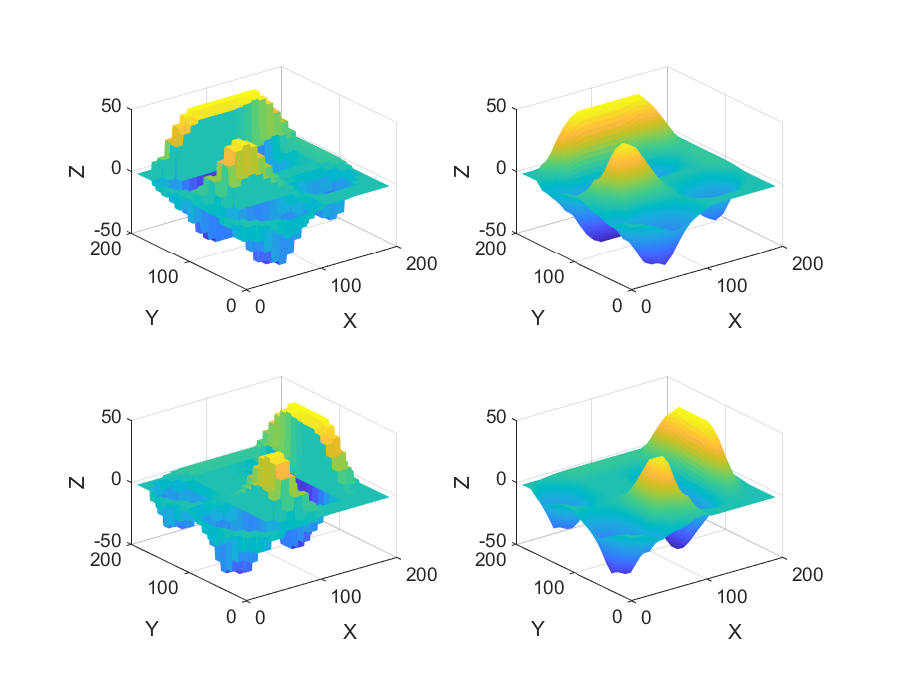
\includegraphics[width=1\linewidth]{non_and_interp_4_plots.eps} 
	\caption{Repulsive field generation via convolutional kernels. Left: Original repulsive fields in X (top) and Y (bottom) directions. Right: Corresponding fields using interpolation, showcasing enhanced smoothness.}
	\label{fig:interp-experiment}
\end{figure}

\section{MANIPULATOR KINEMATICS}

\subsection{INVERSE KINEMATIC CONTROL}

The desired movement of the end-effector is achieved by using inverse kinematics velocity control scheme with task prioritisation. 

\begin{equation}
	\dot{\vec{q}} = \mathbf{J}^+ \xi_{p} \mathrm{\vec{v}{att}} + \dot{\vec{q}}_{rep}
\end{equation}

The damped Moore-Penrose pseudo-inverse, \(\mathbf{J}^+~=~\mathbf{J}'(\mathbf{J}\mathbf{J}' + \sigma_{ee} \mathbf{I})^{-1}\), is utilized to mitigate singularity issues and improve numerical stability in inverse kinematics computations. $\xi_{p}$ is the primary task execution slowdown constant. Finally $\dot{\vec{q}}_{rep}$ are the weighted sum of avoidance joint velocities, each transformed into the null space of primary velocities, as described in the chapter below. 

We run the inverse kinematics algorithm once for every time step, until we reach the desired cost function or reach the selected time limit. 

\subsection{END-EFFECTOR VELOCITY}

Prioritizing control over the end-effector's (EE) translational velocity is essential for a consistent and stable target approach. The commonly used method, where translational velocity is proportional to squared distance, leads to impractically high initial velocities, which can prevent obstacle avoidance and real-world execution, followed by disproportionately slow velocities when nearing the goal position. Our aim is a consistent velocity profile throughout the trajectory, with controlled deceleration near the goal. This is achieved by first calculating the unit vector towards the target for direction, then modulating its magnitude using a sigmoid function, specifically the arctangent function (eq. \ref{eq: v_att}).

\begin{equation} 
	\vec{v} = \frac{\vec{x}_{EE} - \vec{x}_g}{||\vec{x}_{EE} - \vec{x}_g||} \times \frac{\arctan(k_{sigm} \; ||\vec{x}_{EE} - \vec{x}_g||) }{pi/2}
	\label{eq: v_att}
\end{equation}

In Eq.~\ref{eq: v_att}, $\vec{v}$ specifies the end-effector's (EE) translational velocity directed towards the target, integrating both its direction and magnitude. Here, $\vec{x}_{EE}$ represents the EE's current position, and $\vec{x}g$ is the target position, both in Cartesian coordinates. The calculation $\frac{\vec{x}{EE}-\vec{x}g}{||\vec{x}{EE}-\vec{x}g||}$ generates a unit vector pointing towards the target, ensuring targeted movement. The velocity's modulation by the arctangent sigmoid function curtails overshooting by moderating speed in proximity to the target and saturating velocity at a predefined upper limit when distant. The parameter \(k_{sigm}\) in the arctangent function adjusts the curve's steepness, affecting how quickly the end-effector decelerates near the target. A higher \(k_{sigm}\) maintains speed until closer to the target for a sharp deceleration, while a lower value starts slowing down earlier for a gradual approach. 

The current orientation of the end-effector (EE) and its goal orientation are encoded through rotation matrices, \(\mathbf{cR}\) for the current state and \(\mathbf{gR}\) for the goal state. The necessary rotational adjustment is identified through the relative rotation matrix \(\mathbf{dR}\), generated by multiplying \(\mathbf{gR}\) with the transpose of \(\mathbf{cR}\) and then normalizing the outcome (eq. \ref{eq: rot_diff_mat}). This process ensures \(\mathbf{dR}\) accurately represents rotational differences, without the effect of any scaling factors.

\begin{equation}
	\mathbf{dR} = \frac{\mathbf{gR} \cdot \mathbf{cR}^{T}}{||\mathbf{gR} \cdot \mathbf{cR}^{T}||}
	\label{eq: rot_diff_mat}
\end{equation}

To enhance computational efficiency and prevent gimbal lock, the approach transitions from matrix to quaternion representations for precise and efficient rotational velocity adjustments, essential for achieving the target orientation of the EE.

The relative rotation matrix is converted into a quaternion, which is subsequently logarithmically transformed. The resulting quaternion's components, excluding the real part, constitute the rotational error vector \( \vec{\omega} \).

\begin{equation}
	\boldsymbol{dR} \mapsto \boldsymbol{dQ} = a + b \, \vec{i} + c \, \vec{j} + d \, \vec{k}
	\label{eq: quat_mapsto}
\end{equation}

\begin{equation}
	\boldsymbol{dQl} = 2 \cdot \log(\boldsymbol{dQ}) = a_{log} + b_{log} \, \vec{i} + c_{log} \, \vec{j} + d_{log} \, \vec{k}
	\label{eq:quat_log}
\end{equation}

\alert{There needs to be an explanation why log, cite: DMP Quaternions article Žlajpah, Ude}



\begin{equation}
	\vec{\omega} =
	\begin{bmatrix}
		b_{log} \\
		c_{log} \\
		d_{log}
	\end{bmatrix}
	\label{eq:rot_error_vector}
\end{equation}

To get the full velocity of the end effector (EE), \( \mathrm{\vec{v}_{att}} \), we combines translational and rotational velocities, which we scale using proportional gains \( k_v \) and \( k_\omega \).

\begin{equation}
	\mathrm{\vec{v}_{att}} = 
	\begin{bmatrix}
		k_{v} * \vec{v}   \\
		k_{\omega} * \vec{\omega}
	\end{bmatrix}
	\label{eq:ee_velocity}
\end{equation}

Utilizing the mapping into the null space of the primary velocity, it becomes evident that at high velocities of the primary task, there may be an insufficient number of degrees of freedom remaining to safely navigate around obstacles. Consequently, the secondary task, which is aimed at obstacle avoidance, lacks the requisite capability and freedom to operate effectively.

\label{chap:primary slowdown}

To mitigate the dominance of the primary task over the secondary task, a mechanism for the deceleration of the primary task's execution has been implemented. This strategy effectively decreases the velocity of the manipulator towards its primary objective, thereby allocating additional maneuverability for secondary tasks.

\begin{equation}
	\label{eq:slowdown}
	\xi_{p}=
	\frac{1}{1 + \kappa_{\text{sec}} ||v_{\text{Rmax}}||}
\end{equation}

The deceleration factor (eq.~\ref{eq:slowdown}) is determined by the constant \( \kappa_{\text{sec}} \) and the magnitude of the maximum repulsive velocity vectors, which is contingent upon the robot's minimal distance from an obstacle \( v_{\text{Rmax}} \). According to the equation, a small \( v_{\text{Rmax}} \) diminishes the deceleration effect, permitting the uninterrupted execution of the primary task. Conversely, large \( v_{\text{Rmax}} \) enhances the deceleration by reducing the $\xi_{p}$ factor, thereby affording the secondary task increased opportunity for obstacles avoidance motion.


\subsection{AVOIDANCE VELOCITIES}

\begin{figure}
	\centering
	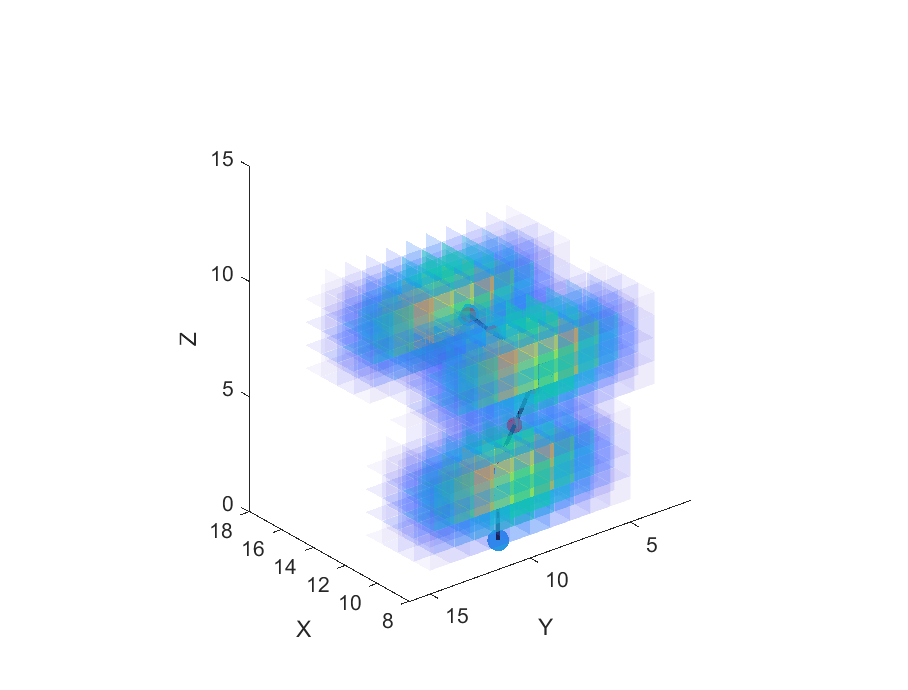
\includegraphics[width=1\linewidth]{manipulator-kernels-visualization-small.eps} % Replace 'example-image' with the filename of your image
	\caption{Visualization of 3 repulsive Y-direction kernels in POI on the manipulator.}
	\label{fig:kernels}
\end{figure}

To enable the avoidance of obstacles by the manipulator within its operating environment, the manipulator is uniformly coated with virtual detection points (POIs). The density of these virtual points is dependent upon the dimensions of matrices. Given a matrix width $w$ perpendicular to the primary direction, it is advantageous for these points to be spaced at intervals of $\Delta = \frac{w}{3}$. This spacing ensures partial overlap between matrices, thereby achieving a uniform distribution of POIs across the entirety of the robot.

During kinematic optimization, repulsive velocities for each point are computed following the methodology described in the previous section (sect. \ref{section:repulsive_vel}). This is achieved by mapping each point into the task space, where the calculation of repulsive velocity is performed. The cartesian mapping for each point comprises a kinematic transformation from the robot's base to the beginning of the segment where the point is located, followed by an additional mapping to the specific point on the segment (eq. \ref{eq:transformations}).  For each point, three components of cartesian velocity are obtained.

\begin{equation}
	\mathbf{T}_{0 \rightarrow \text{POI}} = \mathbf{T}_{0 \rightarrow 1} \cdot \mathbf{T}_{1 \rightarrow 2} \cdot \ldots \cdot \mathbf{T}_{(j-1) \rightarrow j} \cdot \mathbf{T}_{j \rightarrow \text{POI}}	
	\label{eq:transformations}
\end{equation}

Upon obtaining the repulsive velocity for each point, the second norm of each velocity is calculated. For a number of $K$ points where the avoidance velocities are greatest, indicative of closest proximity to an obstacle, the resulting joint velocities that facilitate obstacle avoidance are computed using inverse kinematic equations for the selected points on the manipulator and transformed into the null-space velocities of the primary task.

\begin{equation}
	\mathbf{J}_{d_i}^{+} = \mathbf{N} \mathbf{J}_{d_i}' (\mathbf{J}_{d_i} \mathbf{N} \mathbf{J}_{d_i}' + \sigma_{rep} \mathbf{I})^{-1}, \quad \text{for } i = 1, 2, \ldots, K;
\end{equation}

We calculate the translational velocity Jacobian for each of the $K$ selected points on the robot. Since our interest lies exclusively in the velocity component that directs us away from obstacles, we consequently narrow our operational space to a single dimension. Consequently, the Jacobian, correlating joint space velocities \(q\) with the directional velocity \(d_i\), is represented as \(J_{d_i} = \vec{n}_i^T \mathbf{J}_i\). The normal vector, signifying the desired avoidance velocity, is essentially the unit velocity vector, derived from our matrices as \(\vec{n}_{i} = \frac{\vec{v}_{poi i}}{||\vec{v}_{poi i}||}\). This approach streamlines computational processes by avoiding the necessity for complex matrix inversions, transforming the Jacobian from a matrix to a vector of dimensions \(1 \times n\), where \(n\) signifies the count of joints preceding the POI, thus facilitating more straightforward calculations of repulsive velocities.

\begin{equation}
	\dot{q}_{rep} = k_r \sum_{i=1}^{K} \alpha_i J_{d_i}^{+} \left(v_i - J_{d_i} J^{+} \xi_{p} \vec{v}_{att}\right)
\end{equation}

The overall avoidance joint velocities are obtained through a weighted sum of the avoidance joint velocities for the selected \(K\) nearest points, taking into account the influence of the primary task of manipulator EE movement on the joint velocities.


\section{SIMULATION RESULTS}

\subsection{Repulsive Field Visualization}

We introduce the resultant repulsive field on a two-dimensional map. While analogous principles apply to three-dimensional spaces, visualization of more dimensions is complex. Utilizing our repulsive potential field velocity calculation method, points were sampled across the entire obstacle map as depicted in Figure \ref{fig:example-field}. The prescribed algorithm was executed at each sampled point to derive the repulsive fields along the X and Y axes, which were subsequently visualized as a composite vector field.

\begin{figure}
	\centering
	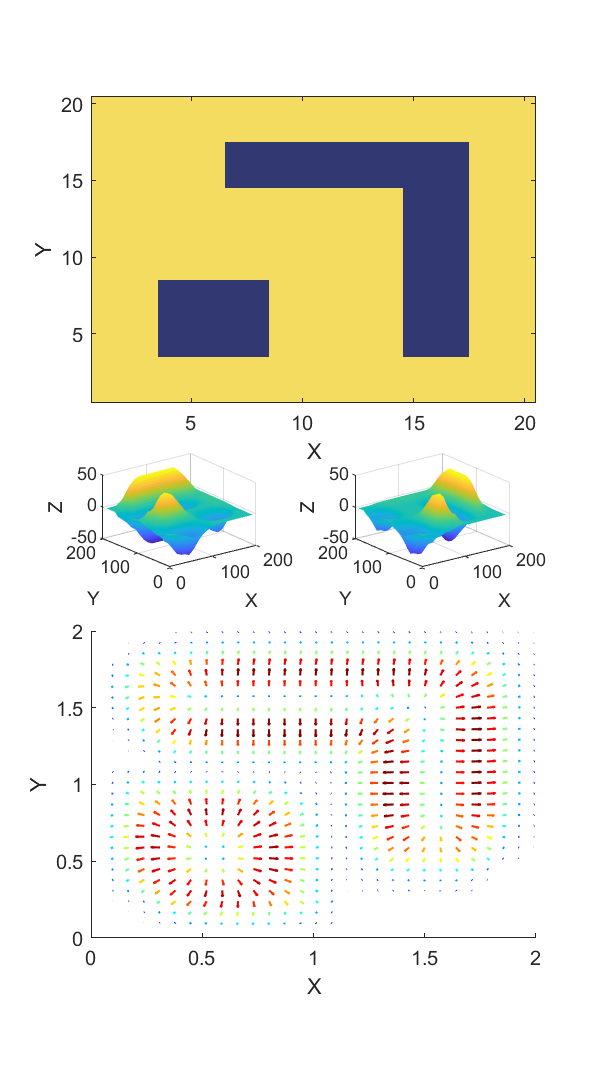
\includegraphics[width=1\linewidth]{demo-field1c.eps} % Replace 'example-image' with the filename of your image
	\caption{Visualization of the potential field calculated for the entire map using the proposed approach. Top: Obstacle distribution via a 2D heatmap. Center: Induced repulsive fields along X (left) and Y (right) axes. Bottom: Composite vector field showcasing the resultant repulsive velocities for obstacle avoidance.}
	\label{fig:example-field}
\end{figure}

\subsection{Manipulator Examples}

The operation of the potential field is demonstrated on two different manipulator cases. The resolution of our voxel grid for obstacles is \( R=10cm \). The use of interpolation allows us to have a relatively coarse voxel grid, which reduces the memory demand of the space grid and accelerates the computation. We selected \( K = 7 \) Points of Interest (POI) to observe the distance from obstacles and are uniformly distributed them along the segments and joints, starting from the second joint of the robot to the tip of the manipulator. This distribution begins from the second joint because it is from this point onwards that the manipulator has the capability to avoid obstacles. Points of Interest (POIs) are indicated by dots on the manipulator in the graphs. Near obstacles, vectors emanate from these points, depicting the calculated repulsive velocities at the locations. Throughout the simulation, Euler integration of the calculated joint velocities is performed with a step size of \( T_{step} = 0.1 \) s.

In the first case (Fig. \ref{fig:keyframes-3d-column}, \ref{fig:plots-3d-column}), the manipulator safely 'curls' or selects a path to a point located on the other side of a column, avoiding the obstacle with the potential field calculated by the proposed method. The constants chosen for the primary task are \( k_v = 5 \) and \( k_w = 1.5 \), for the avoidance task \(k_r=20\). The weighting constants for the individual POIs are \( \alpha = \frac{[ \frac{3}{9}, \frac{2}{9}, \frac{1}{9}, \frac{1}{9}, \frac{1}{9}, \frac{1}{9} ]}{10} \), where the biggest weight belongs to the point on the manipulator which is closest to the obstacle and so on. As the most direct path for the end-effector to the target passes straight through the column, an approach that would result in a collision, we implement a reduction of the primary speed in the vicinity of the obstacle, setting \( \xi_{p} = 1 \). The simulation is performed for 50 steps. 

\begin{figure}
	\centering
	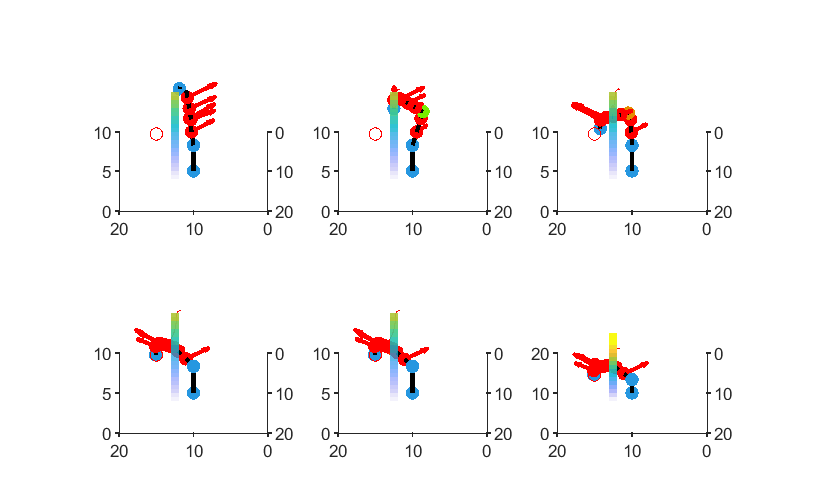
\includegraphics[width=1\linewidth]{keyframes_3D.eps} % Replace 'example-image' with the filename of your image
	\caption{Sequential keyframes demonstrating the manipulator's path planning and column obstacle avoidance strategy.}
	\label{fig:keyframes-3d-column}
\end{figure}


\begin{figure}
	\centering
	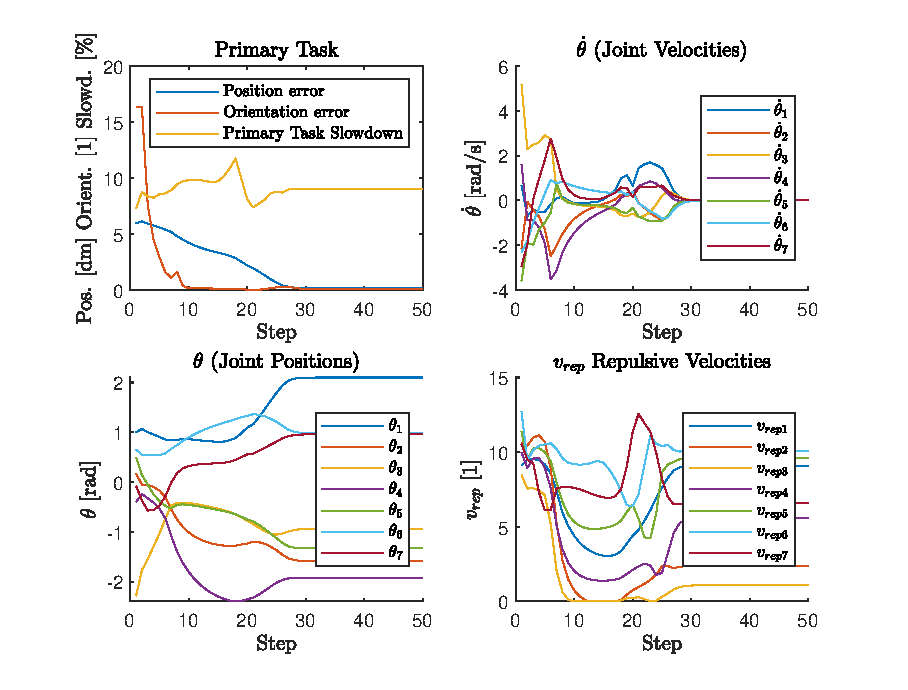
\includegraphics[width=1\linewidth]{4plots_column.eps} % Replace 'example-image' with the filename of your image
	\caption{Visualization of the manipulator's path around the column obstacle: (a) Primary Task errors and percentage of the primary speed after applying slowdown, (b) Joint Velocities $\dot{\theta}$, (c) Joint Positions $\theta$, and (d) Norms of Repulsive Velocities $v_{rep}$.}
	\label{fig:plots-3d-column}
\end{figure}

In the second scenario (Fig. \ref{fig:keyframes-3d-ball}, \ref{fig:plots-ball}), our robot operates within a dynamic environment. The proposed method for calculating repulsive velocities proves to be a suitable choice when a local optimization approach is needed to accommodate dynamic changes. In this scenario, a ball moves consistently from the left to the right side of the graph (i.e., along the y-axis from 0.4 at the initial moment to 1.4 in the final step of the simulation), as governed by the equation \( y_{\text{ball}} = 0.4 + (1.4 - 0.4) \times \frac{N_{\text{step}}}{75} \),  with \( x_{\text{ball}} = 1.25 \) and \( z_{\text{ball}} = 0.7 \). The primary task is now to maintain the robot's end-effector (EE) at a fixed point, disregarding EE orientation to enhance obstacle avoidance capability. This increases maneuverability, thereby eliminating the need for primary speed task slowdown (\( \xi_{p} = 0 \)). Constants selected for the primary task are \( k_v = 2 \) and \( k_w = 0 \), and for the avoidance task \( k_r = 3 \). Weighting constants for the individual POIs are \( \alpha = \frac{[ \frac{1}{5}, \frac{1}{5}, \frac{1}{5}, \frac{1}{5}, \frac{1}{5}, \frac{1}{5} ]}{10} \). The simulation is performed for 75 steps. 

\add{describe weights and distributions used in experiments the kernels}

\add{sigmoid weights}

\begin{figure}
	\centering
	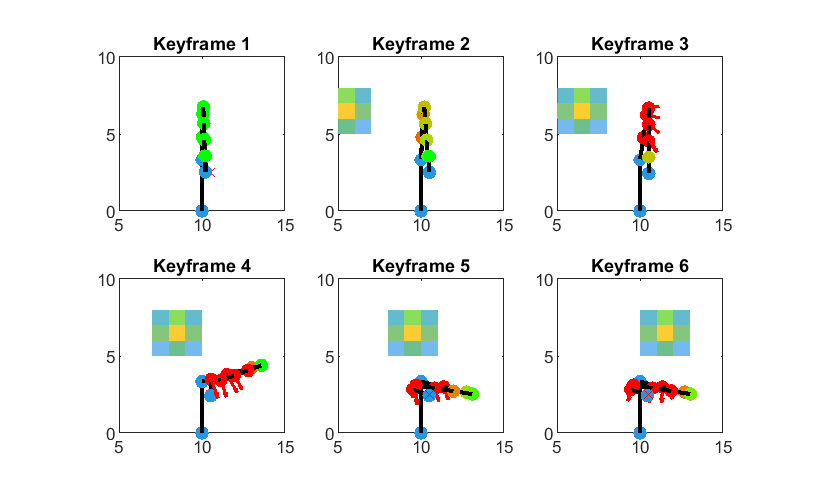
\includegraphics[width=1\linewidth]{keyframes_2D_ball.eps} % Replace 'example-image' with the filename of your image
	\caption{Dynamic obstacle avoidance scenario: Sequential keyframes illustrating the robot’s maneuvering in response to a progressively moving ball from left to right across the workspace.}
	\label{fig:keyframes-3d-ball}
\end{figure}

\begin{figure}
	\centering
	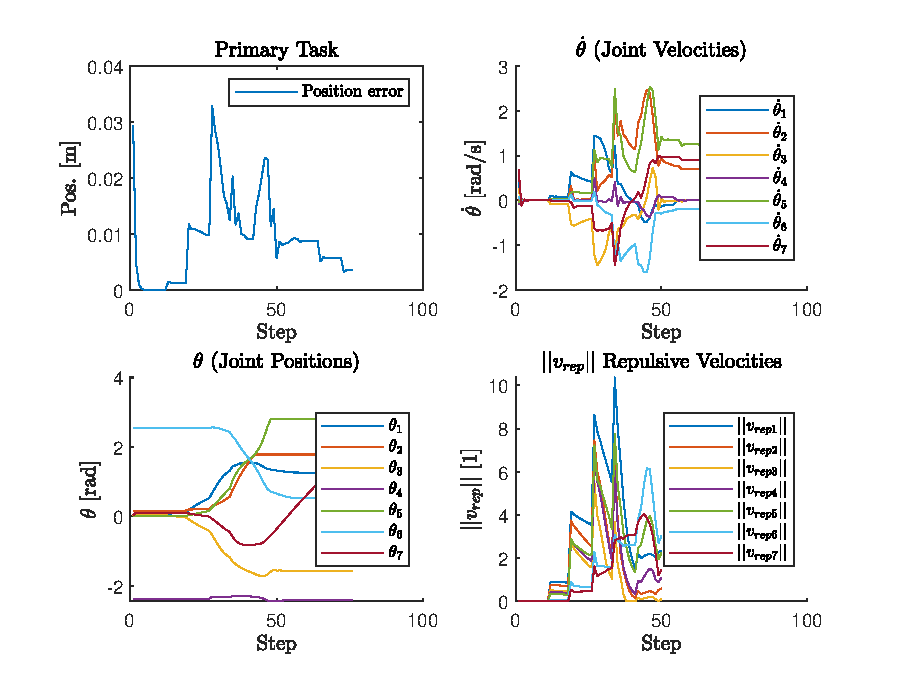
\includegraphics[width=1\linewidth]{4plots_ball.eps} % Replace 'example-image' with the filename of your image
	\caption{Performance in a dynamic obstacle avoidance scenario: (a) Primary Task error (b) Joint Velocities $\dot{\theta}$, (c) Joint Positions $\theta$, and (d) Norms of Repulsive Velocities $v_{rep}$.}
	\label{fig:plots-ball}
\end{figure}
%



\section{CONCLUSION}

\add{ADD}

\addtolength{\textheight}{-12cm}   % This command serves to balance the column lengths
                                  % on the last page of the document manually. It shortens
                                  % the textheight of the last page by a suitable amount.
                                  % This command does not take effect until the next page
                                  % so it should come on the page before the last. Make
                                  % sure that you do not shorten the textheight too much.


\begin{thebibliography}{99}
	
\bibitem{c52} M. G. Tamizi, M. Yaghoubi, and H. Najjaran, “A review of recent trend in motion planning of industrial robots,” Int J Intell Robot Appl, vol. 7, no. 2, Art. no. 2, Jun. 2023. doi: 10.1007/s41315-023-00274-2.
	
\bibitem{siciliano1990kinematic} B. Siciliano, “Kinematic control of redundant robot manipulators: A tutorial,” J. Intell. Robot. Syst., vol. 3, no. 3, Art. no. 3, 1990, doi: 10.1007/BF00126069.

\bibitem{lavalle1998rapidly} S. LaValle, “Rapidly-exploring random trees: A new tool for path planning,” Research Report 9811, 1998.

\bibitem{gammell2015batch} J. D. Gammell, S. S. Srinivasa, and T. D. Barfoot, “Batch Informed Trees (BIT*): Sampling-based Optimal Planning via the Heuristically Guided Search of Implicit Random Geometric Graphs,” in Proc. of the 2015 IEEE International Conference on Robotics and Automation (ICRA), May 2015, pp. 3067–3074. doi: 10.1109/ICRA.2015.7139620.

\bibitem{karaman2010incremental} S. Karaman and E. Frazzoli, "Incremental sampling-based algorithms for optimal motion planning," in Proc. Robotics: Science and Systems (RSS), 2010.

\bibitem{kuffner2000rrt} J. J. Kuffner and S. M. LaValle, “RRT-connect: An efficient approach to single-query path planning,” in Proceedings of the 2000 ICRA. Millennium Conference. IEEE International Conference on Robotics and Automation. Symposia Proceedings (Cat. No.00CH37065), Apr. 2000, pp. 995–1001 vol.2. doi: 10.1109/ROBOT.2000.844730.

\bibitem{c29} A. A. Maciejewski and C. A. Klein, “Obstacle Avoidance for Kinematically Redundant Manipulators in Dynamically Varying Environments,” The International Journal of Robotics Research, vol. 4, no. 3, pp. 109–117, Sep. 1985. doi: 10.1177/027836498500400308.

\bibitem{c38} Y. Nakamura, H. Hanafusa, and T. Yoshikawa, “Task-Priority Based Redundancy Control of Robot Manipulators,” The International Journal of Robotics Research, vol. 6, no. 2, pp. 3–15, Jun. 1987. doi: 10.1177/027836498700600201.

\bibitem{c21} E. A. Basso and K. Y. Pettersen, “Task-Priority Control of Redundant Robotic Systems using Control Lyapunov and Control Barrier Function based Quadratic Programs,” in IFAC-PapersOnLine, vol. 53, no. 2, pp. 9037–9044, 2020. doi: 10.1016/j.ifacol.2020.12.2024.

\bibitem{c23} H. Toshani and M. Farrokhi, “Real-time inverse kinematics of redundant manipulators using neural networks and quadratic programming: A Lyapunov-based approach,” Robotics and Autonomous Systems, vol. 62, no. 6, pp. 766–781, Jun. 2014. doi: 10.1016/j.robot.2014.02.005.

\bibitem{haviland2021neo} J. Haviland and P. Corke, “NEO: A Novel Expeditious Optimisation Algorithm for Reactive Motion Control of Manipulators,” IEEE Robot. Autom. Lett., vol. 6, no. 2, Art. no. 2, Apr. 2021, doi: 10.1109/LRA.2021.3056060.

\bibitem{c44} Z. Long, “Virtual target point-based obstacle-avoidance method for manipulator systems in a cluttered environment,” Engineering Optimization, vol. 52, no. 11, Art. no. 11, Nov. 2020. doi: 10.1080/0305215X.2019.1681986.

\bibitem{c33} O. Khatib, “Real-time obstacle avoidance for manipulators and mobile robots,” in 1985 IEEE International Conference on Robotics and Automation Proceedings, Mar. 1985, pp. 500–505. doi: 10.1109/ROBOT.1985.1087247.

\bibitem{c43} M. F. Pinto, T. R. F. Mendonça, L. R. Olivi, E. B. Costa, and A. L. M. Marcato, “Modified approach using variable charges to solve inherent limitations of potential fields method,” in Proc. 2014 11th IEEE/IAS International Conference on Industry Applications, Dec. 2014, pp. 1–6. doi: 10.1109/INDUSCON.2014.7059414.

\bibitem{c45} A. H. Qureshi and Y. Ayaz, “Potential Functions based Sampling Heuristic For Optimal Path Planning,” Auton Robot, vol. 40, no. 6, Art. no. 6, Aug. 2016. doi: 10.1007/s10514-015-9518-0.

\bibitem{c47} J. Yi, Q. Yuan, R. Sun, and H. Bai, “Path planning of a manipulator based on an improved P\_RRT* algorithm,” Complex Intell. Syst., vol. 8, no. 3, pp. 2227–2245, Jun. 2022. doi: 10.1007/s40747-021-00628-y.

\bibitem{klancar2022robot}
G. Klančar, A. Zdešar, and M. Krishnan, “Robot Navigation Based on Potential Field and Gradient Obtained by Bilinear Interpolation and a Grid-Based Search,” Sensors, vol. 22, no. 9, art. no. 3295, pp. 1-24, 2022. doi: 10.3390/s22093295.

\bibitem{c49} X. Xia et al., “Path Planning for Obstacle Avoidance of Robot Arm Based on Improved Potential Field Method,” Sensors, vol. 23, no. 7, Art. no. 7, Apr. 2023. doi: 10.3390/s23073754.

\bibitem{park2020trajectory} S.-O. Park, M. C. Lee, and J. Kim, “Trajectory Planning with Collision Avoidance for Redundant Robots Using Jacobian and Artificial Potential Field-based Real-time Inverse Kinematics,” Int. J. Control Autom. Syst., vol. 18, no. 8, Art. no. 8, Aug. 2020, doi: 10.1007/s12555-019-0076-7.

\bibitem{baumgartner2023potential}
J. Baumgartner, T. Petrič, and G. Klančar, “Potential Field Control of a Redundant Nonholonomic Mobile Manipulator with Corridor-Constrained Base Motion,” Machines, vol. 11, no. 2, art. no. 293, pp. 1-28, 2023. doi: 10.3390/machines11020293.

\bibitem{oleynikova2017voxblox} H. Oleynikova, Z. Taylor, M. Fehr, R. Siegwart, and J. Nieto, “Voxblox: Incremental 3D Euclidean Signed Distance Fields for on-board MAV planning,” in Proc. of the 2017 IEEE/RSJ International Conference on Intelligent Robots and Systems (IROS), Vancouver, BC, Sep. 2017, pp. 1366–1373. doi: 10.1109/IROS.2017.8202315.

\bibitem{han2019fiesta} L. Han, F. Gao, B. Zhou, and S. Shen, “FIESTA: Fast Incremental Euclidean Distance Fields for Online Motion Planning of Aerial Robots,” arXiv, Jul. 26, 2019. Accessed: Jan. 11, 2024. [Online]. Available: http://arxiv.org/abs/1903.02144

\bibitem{lau2010improved} B. Lau, C. Sprunk, and W. Burgard, “Improved updating of Euclidean distance maps and Voronoi diagrams,” in Proc. of the 2010 IEEE/RSJ International Conference on Intelligent Robots and Systems, Taipei, Oct. 2010, pp. 281–286. doi: 10.1109/IROS.2010.5650794.

\bibitem{rong2006jump} G. Rong and T.-S. Tan, “Jump flooding in GPU with applications to Voronoi diagram and distance transform,” in Proceedings of the 2006 Symposium on Interactive 3D Graphics and Games - SI3D ’06, Redwood City, California, 2006, p. 109. doi: 10.1145/1111411.1111431.

\bibitem{zhou2021egoplanner} X. Zhou, Z. Wang, H. Ye, C. Xu, and F. Gao, “EGO-Planner: An ESDF-Free Gradient-Based Local Planner for Quadrotors,” IEEE Robot. Autom. Lett., vol. 6, no. 2, pp. 478–485, Apr. 2021, doi: 10.1109/LRA.2020.3047728.

\bibitem{han2018dynamic} D. Han, H. Nie, J. Chen, and M. Chen, “Dynamic obstacle avoidance for manipulators using distance calculation and discrete detection,” Robotics and Computer-Integrated Manufacturing, vol. 49, pp. 98–104, Feb. 2018, doi: 10.1016/j.rcim.2017.05.013.

\bibitem{c30} L. Žlajpah and T. Petrič, “Obstacle Avoidance for Redundant Manipulators as Control Problem,” in Serial and Parallel Robot Manipulators - Kinematics, Dynamics, Control and Optimization, S. Kucuk, Ed. InTech, 2012. doi: 10.5772/32651.

\bibitem{c32} K. Glass, R. Colbaugh, D. Lim, and H. Seraji, “Real-time collision avoidance for redundant manipulators,” IEEE Trans. Robot. Automat., vol. 11, no. 3, pp. 448–457, Jun. 1995. doi: 10.1109/70.388789.

\bibitem{c41} L. Žlajpah and B. Nemec, “Kinematic control algorithms for on-line obstacle avoidance for redundant manipulators,” in Proc. IEEE/RSJ International Conference on Intelligent Robots and Systems, Lausanne, Switzerland, 2002, pp. 1898–1903. doi: 10.1109/IRDS.2002.1044033.


\end{thebibliography}




\end{document}
